\documentclass[a4paper]{article}

\usepackage[utf8]{inputenc}
% \usepackage[fontset=ubuntu]{ctex}
\usepackage{ctex}
\usepackage[ruled,linesnumbered]{algorithm2e}
\usepackage{xcolor}
\usepackage{amsmath}
\usepackage{graphicx}
\usepackage{listings}
\usepackage{verbatim}
\usepackage{bigints}
\usepackage{amsmath}
\usepackage{float}
\usepackage{titling}
\usepackage[colorinlistoftodos]{todonotes}

\definecolor{codegreen}{rgb}{0,0.6,0}
\definecolor{codegray}{rgb}{0.5,0.5,0.5}
\definecolor{codepurple}{rgb}{0.58,0,0.82}
\definecolor{backcolour}{rgb}{0.95,0.95,0.92}

\lstdefinestyle{mystyle}{
    backgroundcolor=\color{backcolour},   
    commentstyle=\color{codegreen},
    keywordstyle=\color{magenta},
    numberstyle=\tiny\color{codegray},
    stringstyle=\color{codepurple},
    basicstyle=\ttfamily\footnotesize,
    breakatwhitespace=false,         
    breaklines=true,                 
    captionpos=b,                    
    keepspaces=true,                 
    numbers=left,                    
    numbersep=5pt,                  
    showspaces=false,                
    showstringspaces=false,
    showtabs=false,                  
    tabsize=2
}

\lstset{style=mystyle}

\title{周报写作模板}

\author{作者}

\date{\today}

\begin{document}
\maketitle

\section{写在前面}

这里来写下前言

\section{算法与代码}
算法使用下面这种格式

\begin{algorithm}[H]
\SetAlgoLined
\KwResult{Write here the result }
 initialization\;
 \While{While condition}{
  instructions\;
  \eIf{condition}{
   instructions1\;
   instructions2\;
   }{
   instructions3\;
  }
 }
 \For{condition}{statement\;}
 
 \caption{How to write algorithms}
\end{algorithm}


代码插入以Python为例
\begin{lstlisting}[language=Python, caption=Python example]
import numpy as np
    
def incmatrix(genl1,genl2):
    m = len(genl1)
    n = len(genl2)
    M = None #to become the incidence matrix
    VT = np.zeros((n*m,1), int)  #dummy variable
    
    #compute the bitwise xor matrix
    M1 = bitxormatrix(genl1)
    M2 = np.triu(bitxormatrix(genl2),1) 

    for i in range(m-1):
        for j in range(i+1, m):
            [r,c] = np.where(M2 == M1[i,j])
            for k in range(len(r)):
                VT[(i)*n + r[k]] = 1;
                VT[(i)*n + c[k]] = 1;
                VT[(j)*n + r[k]] = 1;
                VT[(j)*n + c[k]] = 1;
                
                if M is None:
                    M = np.copy(VT)
                else:
                    M = np.concatenate((M, VT), 1)
                
                VT = np.zeros((n*m,1), int)
    
    return M
\end{lstlisting}


\section{插图}
插图使用例

\begin{figure}[H]
\centering
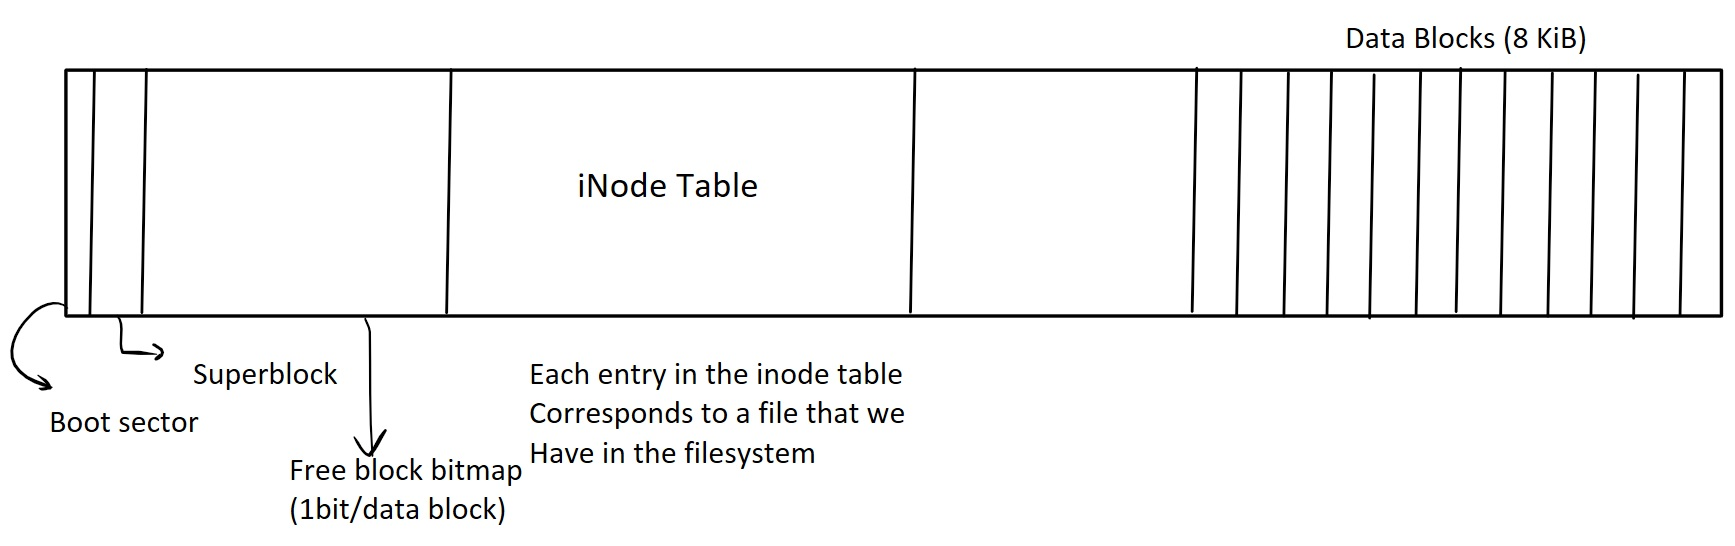
\includegraphics[width=0.75\textwidth]{img/sample.jpg}
\caption{\label{fig:BLayout}例图}
\end{figure}

\subsection{子小节}

子小节内容,可以这样\textbf{加粗}

\subsection{分点并列}

并列的点使用下面这种格式

\begin{itemize}
\item 分点1
\item 分点2
\item 分点3
\end{itemize}

需要使用分小块详细介绍时这样做

\begin{enumerate}
\item \textbf{内容1}: 内容
\item \textbf{内容2}: 内容
\end{enumerate}

\subsubsection{公式} 
可以插入行内公式,如$a+b = c$。
也可以插入行间公式,如
\begin{align*}
\bigintss_0^1 \left( \dfrac{\int_0^h (h-i)di}{h} + \dfrac{\int_h^1 (i-h)di}{1-h} \right) dh
\end{align*}
上面是一个行间公式。

\section{引用说明}
需要引用时这样做\cite{szegedy2015going},例如介绍ResNet\cite{he2016deep}以及ImageNet\cite{russakovsky2015imagenet}数据集时进行引用。

%自动列出已引用的参考文献部分
\bibliographystyle{ieeetr}
\bibliography{ref}

\end{document}